The main purpose of this paper is to present the reader with some instances of neural networks in order to predict the price of a stock (S\&P500, Tesla, Facebook...).

Let's first define what a neural network is, and in very general terms, how it learns.

\section{Deep Neural Network Model}
A deep neural network is usually represented with the diagram present in \hyperref[fig:NNGeneral]{Figure 1.1}

\begin{figure}[h]
    \centering
    \begin{neuralnetwork}[height=4]
		\newcommand{\nodetextx}[2]{$x_#2^{(0)}$}
		\newcommand{\nodetexth}[2]{$x_#2^{(1)}$}
		\newcommand{\nodetexthh}[2]{$x_#2^{(2)}$}
		\newcommand{\nodetexto}[2]{$x_#2^{(3)}$}
		\inputlayer[count=3, bias=false, title=Input\\layer, text=\nodetextx]
		\hiddenlayer[count=4, bias=false, title=Hidden\\layer, text=\nodetexth] \linklayers 
        \hiddenlayer[count=4, bias=false, title=Hidden\\layer, text=\nodetexthh] \linklayers
        \outputlayer[count=1, bias=false, title=Output\\layer,
        text=\nodetexto] \linklayers
    \end{neuralnetwork}
    \caption{General Deep Neural Network Model}
    \label{fig:NNGeneral}
\end{figure}
We have the standard model with input layer which takes in the data as input, a series of hidden layers which transform the data until we get to the output layer which will produce the stock prediction we are looking for.

\textbf{Neurons}: The notation of our neurons will be $x_i^{(j)}$ which refers to the $i$-th neuron in layer $j$.

\section{Propagation Function}
The output of each neuron is calculated using a propagation function, firstly every neuron has $n$ inputs and $1$ output, if we take a look at a reduced model like the one in \hyperref[fig:PropFunct]{Figure 1.2}

\begin{figure}[h]
    \centering
    \begin{tikzpicture}[roundnode/.style={circle, draw=black!60, fill=gray!5, very thick, minimum size=7mm}]
        \node[roundnode] (1) {$x_0^{(0)}$};
    \node[roundnode] (2) [below=of 1] {$x_1^{(0)}$};
    \node[roundnode] (3) [right=of 2] {$x_0^{(1)}$};
    \node[roundnode] (4) [below=of 2] {$x_n^{(0)}$};
    
    \draw [->](1) -- (3) node [midway, above, sloped] (TextNode) {$w_{0,0}$};
    \draw [->](2) -- (3) node [midway, above, sloped] (TextNode) {$w_{0,1}$};
    \draw [->](4) -- (3) node [midway, above, sloped] (TextNode) {$w_{0,2}$};
    \draw [->] (3) -- (4,-2.2) node [midway, above, sloped] (TextNode) {$x_0^{(1)}$};

    \end{tikzpicture}
    \caption{Caption}
    \label{fig:my_label}
\end{figure}

We have that the value of $x_0^{(1)}$ is defined from the following equation
\begin{equation}
    x_0^{(1)} = \sigma\left(w_{0,0}x_0^{(0)} + w_{0,1}x_1^{(0)} + w_{0,2}x_2^{(0)} + b_0\right)
\end{equation}
Where
\begin{itemize}
    \item $sigma$ is an activation function, normally non-linear such as the sigmoid, hyperbolic tangent, but depending on the model it can also be ReLU (rectified linear).
    \item $w_{i,j}$ is the weight between neuron $j$ and neuron $i$ of the next layer.
    \item $b_0$ is the bias term
\end{itemize}

So if we generalize for $n$ inputs we have the analogous formula
\begin{align}
    x_0^{(1)} &= \sigma\left(w_{0,0}x_0^{(0)} + w_{0,1}x_1^{(0)} + ... + w_{0,n}x_n^{(0)} + b_0\right) \\
    &= \sigma\left(
    \begin{bmatrix}
    w_{0,0} &  w_{0,1} & ... & w_{0,n}
    \end{bmatrix}
    \begin{bmatrix}
    x_0^{(0)}\\ x_1^{(0)}\\ ... \\ x_n^{(0)}
    \end{bmatrix} + b_0
    \right)
\end{align}
We can generalize it further by observing the formula to calculate the outputs of a whole layer of $k$ neurons from the $n$ outputs of the previous layer's nodes.
\begin{equation}
    \begin{bmatrix}
    x_0^{(1)}\\ x_1^{(1)}\\ ... \\ x_k^{(1)}
    \end{bmatrix} = \sigma\left(
    \begin{bmatrix}
    w_{0,0} &  w_{0,1} & ... & w_{0,n} \\
     w_{1,0} &  w_{1,1} & ... & w_{1,n} \\
     ... & ... & ... & ... \\
     w_{k,0} &  w_{k,1} & ... & w_{k,n} 
    \end{bmatrix}
    \begin{bmatrix}
    x_0^{(0)}\\ x_1^{(0)}\\ ... \\ x_n^{(0)}
    \end{bmatrix} + \begin{bmatrix}
    b_0\\ b_1\\ ... \\ b_n
    \end{bmatrix}
    \right)
\end{equation}

\subsection{Activation Function}
We can take a closer look at the mentioned activation functions


\begin{minipage}{\linewidth}
      \centering
      \begin{minipage}[t]{0.32\linewidth}
          \begin{figure}[H]
                 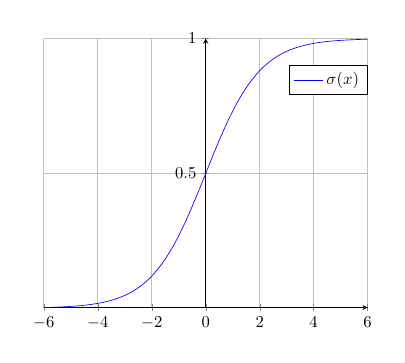
\begin{tikzpicture}[scale=0.6, declare function={sigma(\x)=1/(1+exp(-\x));
        sigmap(\x)=sigma(\x)*(1-sigma(\x));}]
        \begin{axis}%
        [
            grid=major,     
            xmin=-6,
            xmax=6,
            axis x line=bottom,
            ytick={0,.5,1},
            ymax=1,
            axis y line=middle,
            samples=100,
            domain=-6:6,
            legend style={at={(1,0.9)}}     
        ]
            \addplot[blue,mark=none]   (x,{sigma(x)});
            \legend{$\sigma(x)$}
        \end{axis}
    \end{tikzpicture}
    
              \caption{\footnotesize{Sigma Activation}}
          \end{figure}
      \end{minipage}
      \begin{minipage}[t]{0.32\linewidth}
          \begin{figure}[H]
            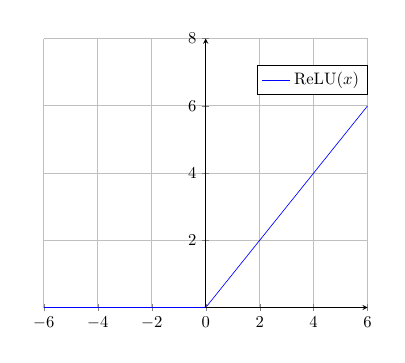
\begin{tikzpicture}[scale=0.6,declare function={relu(\x)=max(x, 0);
        relup(\x)=relu(\x) / \x;}]
        \begin{axis}%
        [
            grid=major,     
            xmin=-6,
            xmax=6,
            axis x line=bottom,
            ymax=8,
            axis y line=middle,
            samples=100,
            domain=-6:6,
            legend style={at={(1,0.9)}}     
        ]
            \addplot[blue,mark=none]   (x,{relu(x)});
            \legend{ReLU$(x)$}
        \end{axis}
    \end{tikzpicture}              
    \caption{Relu Activation}
          \end{figure}
      \end{minipage}
      \begin{minipage}[t]{0.32\linewidth}
      \begin{figure}[H]
          \begin{tikzpicture}[scale=0.6, declare function={tanhp(\x)=1 - tanh(x)^2;}]
        \begin{axis}%
        [
            grid=major,     
            xmin=-6,
            xmax=6,
            axis x line=middle, bottom,
            ytick={-1,-.5,0,.5,1},
            ymax=1,
            axis y line=middle,
            samples=100,
            domain=-6:6,
            legend style={at={(1,0.9)}}     
        ]
            \addplot[blue,mark=none]   (x,{tanh(x)});
            \legend{$\tanh(x)$}
        \end{axis}
    \end{tikzpicture}
    \caption{tanh Activation}
    \end{figure}
      \end{minipage}
  \end{minipage}

We want a non-linear activation function, since if we chose a linear one, our whole deep model would be reducible into a linear neural network with 1 layer.

\section{Learning}
Now, in order to adjust our model's weight so they correctly give accurate predictions, we must train our neural network, we will do so in a \textbf{supervised} manner, that is, from a know dataset of (features, label) we will input these features into our model and compare the output we get with the true output (label), we need to define a \textbf{loss function} to compute the difference between the two, most commonly we will use the \textit{squared loss function}
\begin{equation}
    l(\textbf{x}) = \|y - h(\textbf{x})\|^2
\end{equation}
where
\begin{itemize}
    \item  $\textbf{x}$: vector of input features
    \item $y$: true output
    \item $h(\textbf{x})$: the output of the neural network for input $\textbf{x}$
\end{itemize}
Since our model's parameters are the weights and biases of the different connections between neurons, and not the dataset, which will be fixed, we can rewrite this loss function in terms of them as
\begin{equation*}
    l(\mathbf{W,b}) = \| y - h_{\mathbf{W,b}}(x) \|^2
\end{equation*}
where 
\begin{itemize}
    \item $h_{\mathbf{W,b}}(x)$: the output of the neural network with set of weights and biases $\mathbf{W}$ and $\mathbf{b}$ respectively, for input $\textbf{x}$ 
\end{itemize}


And therefore the expression of the error over an entire dataset consisting of $n$ pairs of (features, label) will be the average of the errors of the $n$ pairs.
\begin{equation*}
    L(\textbf{x}) = \frac{1}{n}\sum_{i=0}^{n} l(\textbf{x}) 
\end{equation*}
And again rewriting for the weights as parameters.
\begin{equation*}
    L(\textbf{W,b}) = \frac{1}{n}\sum_{i=0}^{n} l(\textbf{W,b}) 
\end{equation*}

When we train our model we will be aiming to minimize this loss function, let's see which are the most common update rules for the weights in order to achieve this.

Firstly, the weights will be initialized randomly, there are a few options, for a set of $n$ features and 1 output we have,
\begin{itemize}
    \item \textbf{Xavier Normal}: we will initialize the weights by sampling them from a Normal distribution with mean 0, and variance $\frac{2}{n+1}$
    \begin{equation*}
        w_{i,j} \sim N\left(0, \frac{2}{\sqrt{n+1}} \right)
    \end{equation*}
    \item \textbf{Xavier Uniform}: The weights follow a uniform distribution
     \begin{equation*}
        w_{i,j} \sim U\left[-\sqrt{\frac{6}{n+1}},\sqrt{\frac{6}{n+1}} \right]
    \end{equation*}
    \item \textbf{He}: Especially used with ReLU activation functions
    \begin{equation*}
        w_{i,j} \sim N\left(0, \frac{2}{n} \right)
    \end{equation*}
\end{itemize}
Now the way to train any deep neural network is to  solve the following optimization problem
\begin{equation}
    \mathbf{\tilde{W}, \tilde{b}} = \underset{\mathbf{W, b}}{argmin} \; L(\mathbf{W, b})
\end{equation}
where
\begin{itemize}
    \item $\mathbf{W}$: set of all weights of a neural network model, spanning all the layers
    \item $\mathbf{b}$: set of all biases of a neural network model
\end{itemize}
Which just means we have to find the appropiate set of weights () and biases ($\mathbf{b}$) that minimize the total error function of the model over a given dataset.

\subsection{Update Rule}
The way to solve this optimization problem is very rarely an analytic solution, so we will iteratively update the weights and biases of our model to reduce the total error, we will use \textit{gradient descent} which is just an algorithm which on every iteration will update the weights in the direction that lowers the error function the most.
\begin{equation}
    \label{eq:gradDescent}
    \mathbf{W,b} := \mathbf{W,b} - \mu * \partial L(\mathbf{W,b})
    \tag{Gradient Descent}
\end{equation}
where $\mu$ is the \textbf{learning rate} or the step of every iteration of the optimization algorithm

If a given dataset is large doing the derivative for the whole dataset is very costly, so we will use a version of \textit{gradient descent} called \textit{minibatch stochastic gradient descent} in which we simply take mini batches of the whole dataset and updating the weight using those batches, the corresponding update rule for a batch $B$ looks like 
\begin{equation}
    \label{eq:gradDescentMini}
    \mathbf{W,b} := \mathbf{W,b} - \mu * \partial L_{B}(\mathbf{W,b})
    \tag{Gradient Descent}
\end{equation}
where $L_B$ is the total error of the model over the batch we are considering ($B$) instead of the whole model.

\section{Vanishing and Exploding Gradient Problem}
When we update our models weights we might run into a few problems which will slow our model's convergence to an optimal solution, or make it impossible for it to arrive to said solution, namely, we will take a look at vanishing gradient and exploding gradient problems.

Suppose we have a deep neural network with $l$ layers, then if we express the layers as $H^{(i)}$ where $H^{(0)}$ is the input layer and $H^{(l)}$ is the output layer, then we can express the value of each layer from the previous one as
\begin{equation*}
    H^{(i)} = f\left( H^{(i-1)} \right)
\end{equation*}
where $f$ is the activation function

Then the output can be expressed as
\begin{equation*}
    H^{(l)} = f \circ f \circ ... \circ f \left(H^{(0)}\right)
\end{equation*}

And the gradient of the output which we will use in the update rule is
\begin{equation*}
    \partial H^{(l)} = \partial f \left(H^{(l-1)}\right) \cdot \partial f \left(H^{(l-2)}\right)\cdot ... \cdot \partial f \left(H^{(0)}\right)
\end{equation*}

Now if we recall the plot of both the sigmoid and tanh activation functions, we can add the plot for their gradients which are
\begin{multicols}{2}
\noindent
\begin{align*}
    \partial \sigma (x) = \frac{\sigma(x)}{1-\sigma(x)}
\end{align*}
\columnbreak
\begin{align*}
    \partial \tanh(x) = \frac{1}{1-\tanh(x)^2}
\end{align*}
\end{multicols}

\begin{minipage}{\textwidth}
      \centering
      \begin{minipage}[t]{0.45\linewidth}
          \begin{figure}[H]
                 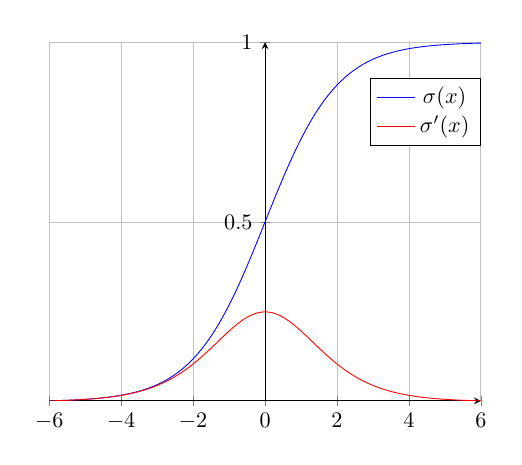
\begin{tikzpicture}[scale = 0.8, declare function={sigma(\x)=1/(1+exp(-\x));        sigmap(\x)=sigma(\x)*(1-sigma(\x));}]
        \begin{axis}%
        [
            grid=major,     
            xmin=-6,
            xmax=6,
            axis x line=bottom,
            ytick={0,.5,1},
            ymax=1,
            axis y line=middle,
            samples=100,
            domain=-6:6,
            legend style={at={(1,0.9)}}     
        ]
            \addplot[blue,mark=none]   (x,{sigma(x)});
            \addplot[red,mark=none]   (x,{sigmap(x)});
            \legend{$\sigma(x)$,$\sigma'(x)$}
        \end{axis}
    \end{tikzpicture}
    \caption{\footnotesize{Sigma activation and it's gradient}}
    \end{figure}
    \end{minipage}
      \begin{minipage}[t]{0.45\linewidth}
      \begin{figure}[H]
          \begin{tikzpicture}[scale = 0.8, declare function={tanhp(\x)=1 - tanh(x)^2;}]
        \begin{axis}%
        [
            grid=major,     
            xmin=-6,
            xmax=6,
            axis x line=middle, bottom,
            ytick={-1,-.5,0,.5,1},
            ymax=1,
            axis y line=middle,
            samples=100,
            domain=-6:6,
            legend style={at={(1,0.9)}}     
        ]
            \addplot[blue,mark=none]   (x,{tanh(x)});
            \addplot[red,mark=none]   (x,{tanhp(x)});
            \legend{$\tanh(x)$, $\tanh'(x)$}
        \end{axis}
    \end{tikzpicture}
    \caption{\footnotesize{tanh activation and it's gradient}}
    \end{figure}
      \end{minipage}
  \end{minipage}

We can see that both gradients are very close to 0  when the input values are small or large, which means that over, $l$ layers the product of values close to 0 will be inevitably close to 0, which if we observe the \hyperref[eq:gradDescent]{gradient descent update rule} means that our model won't update the weights and therefore will be stuck.

Exploding gradient is the opposite, when the gradients value, is large so after the product of $l$ layers of gradients, this will result in our weights (and biases) suffering very large updates which prevent our model from converging correctly to a solution.

\subsection{Solutions}
The exploding gradient can be solved by using sigmoid or tanh activation functions, but these functions still suffer from the vanishing gradient problem. So the solution is to use ReLU activation function
\begin{figure}[H]
    \centering
    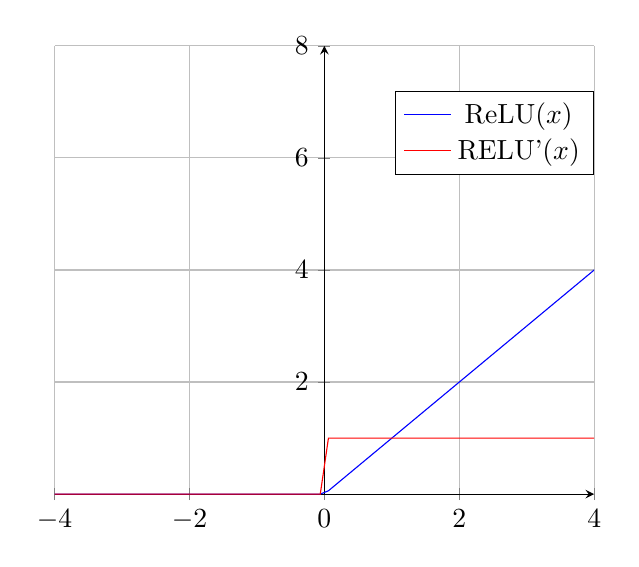
\begin{tikzpicture}[declare function={relu(\x)=max(x, 0);
        relup(\x)=relu(\x) / \x;}]
        \begin{axis}%
        [
            grid=major,     
            xmin=-4,
            xmax=4,
            axis x line=bottom,
            ymax=8,
            axis y line=middle,
            samples=100,
            domain=-6:6,
            legend style={at={(1,0.9)}}     
        ]
            \addplot[blue,mark=none]   (x,{relu(x)});
            \addplot[red,mark=none] (x, {relup(x)});
            \legend{ReLU$(x)$, RELU'$(x)$}
        \end{axis}
    \end{tikzpicture}             
    \caption{ReLU activation function and it's gradient}
    \label{fig:relu}
\end{figure}

Now we won't have the problem of a gradient vanishing, since the gradient is either 0 or 1. The only problem ReLu poses is that if one of the neurons has gradient 0 then the whole gradient of the update will also be 0 meaning we won't update the weights, to solve this we can use a special version of ReLu, such as \textbf{leaky ReLu} where the gradient of the function is not exactly 0 when the input is less than 0.

Another option is to use \textbf{LSTM Neural Networks} which, by their architecture, which is briefly explained in TODO PONER EL CAPITULO DE LTSM, the input gate, which if turned off preserves the long term dependencies and allows them to be learnt.